\documentclass[11pt, twocolumn]{article}

\usepackage{themeKonstanz} 

% Thesis information  %
\date{\today}
\year{2022}
\author{Fabian Klopfer}
\title{Multi-Electrode Array Local Field Potential Analysis Toolbox}
\uni{University of Tübingen}
\unisection{Faculty of Medicine}
\department{Graduate Training Centre of Neuroscience}
\track{Neural \& Behavioral Science}
\institute{Hertie Institute for Clincal Brain Research \\ University Hospital Tübingen}
\supervisorOne{Dr. Thomas Wuttke}
\supervisorTwo{Dr. Ulrike Hedrich}

\headFoot{14}
 
\bibliography{resources} 


\begin{document}
\thesistitlepage[language=english]
    \newgeometry{left=2.5cm, right=2.5cm, bottom=2cm, top=2.5cm, headheight=14pt, headsep=0.8cm, footskip=30pt}
\twocolumn[

  \begin{@twocolumnfalse}

    \begin{abstract}
In the context of epilepsy and migraine caused by channelopathies, electrophysiological data is crucial for research. Besides single cell recording, network-wide data is neccessary for insights about the emergence and spreading of these pathologies.
One way to gather network-level data is to record neural activity from brain slices with a micro-electrode array.
The analysis of such-recorded local field potentials requires careful consideration of the set-up parameters like electrode distance and probe properties. Existing software fails to fullfill all requirements imposed by the task and its context. Thus we implemented a toolbox which meets these and present the work in this report.
\end{abstract}
\vspace*{5cm}
\tableofcontents
  \end{@twocolumnfalse}
]

\restoregeometry
\rmfamily 
\normalsize

\section{Introduction}
    \subsection{Motivation}
        Mutations in ion channals expressed in neurons can cause a wide range of pathological behaviors.
        These are called channelopathies.
        Mutations to a specific channel, the voltage-gated sodium channel 1.1 (Na$_V$1.1), can cause both epileptic and migraine phenotypes.
        While epilepsy causes seizures, migraine causes a wavefront of increased depolarization followed by a temporary decrease in neural depolarization.
        To investigate this phenomenon, micro-electrode arrays can be used to record neural activity on a network level for both models and a baseline/wild type group, yielding local field potentials.
        The so obtained recordings capture multi-unit activity which needs to be analyzed carefully with the scale of the local field potentials in mind.
        As existing software fails to provide a framework that matches the scale of the local field potentials, is proprietary and vendor specific, or quality-wise insufficient, there is a need for a tailored solution that semi-automatizes parts of the data analysis in a user-oriented way. \\

        During the lab rotation I implemented a solution to the above problem.
        In the next section, local field potentials, micro-electrode arrays and existing software systems are described with respect to the context of the lab rotation.
        Next the task is specified along with the implemented solution. The final part of this report discusses limitations of and future directions for the presented solution.
\section{Background}
    \subsection{Local Field Potentials}
        Neural activity induces changes in the concentration of ions across the cell membrane and gradients among different compartment of the neuron and between neurons, as shown in figure \ref{field}.
        \begin{figure}
        \begin{center}
         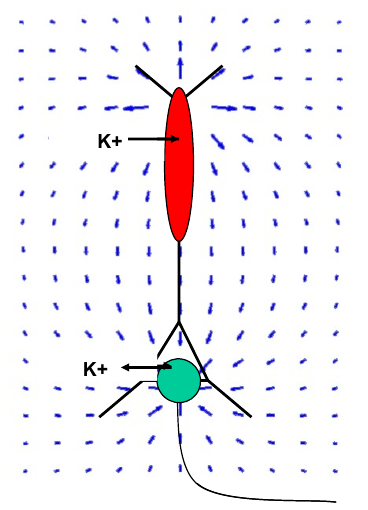
\includegraphics[keepaspectratio, width=0.3\textwidth]{img/2_lfp.png}
        \end{center}
         \caption{A visualization of how an electrical field is created by a single neuron. When an action potential is fired, potassium channels open and potassium flows out of the cell. Na$^+$/K$^+$-ATPases pump K$^+$ ions back in. These two processes together with the temporal delay between channel opening in different compartments create the necessary soruce and sink for the electrical field.}\label{field}
        \end{figure}

        These changes induce an electrical field which can be measured extracellularly using electrodes.
        The high frequency components above $~500$ Hz of this signal is closely related to the spiking activity of neurons in close vincity of the electrode.
        Lower frequency parts of the signal are  called local field potentials (LFPs), which do not allow for an as straight forward interpretation when it comes to the underlying neural activity~\autocite{einevoll2013modelling, herreras2016local}.
        LFPs can be meassured on different scales ranging from single unit recordings over multi unit recordings with different setups (e.g. multi-electrode arrays vs. deep brain electrodes) up to extra-cranial recordings, placing the electrode on the skin head. \\

        The different scales require each a different Ansatz for analysis and interpretation:
        While single unit recordings (SUR) allow to track action potentials (APs), multi-unit recordings (MUR) capture aggregated neural activity of populations. Aggregation means, that the meassured voltage differences are caused by many different neurons, as visualized and explained in figures \ref{mur} and \ref{origins}
        \begin{figure}
        \begin{subfigure}{0.45\textwidth}
         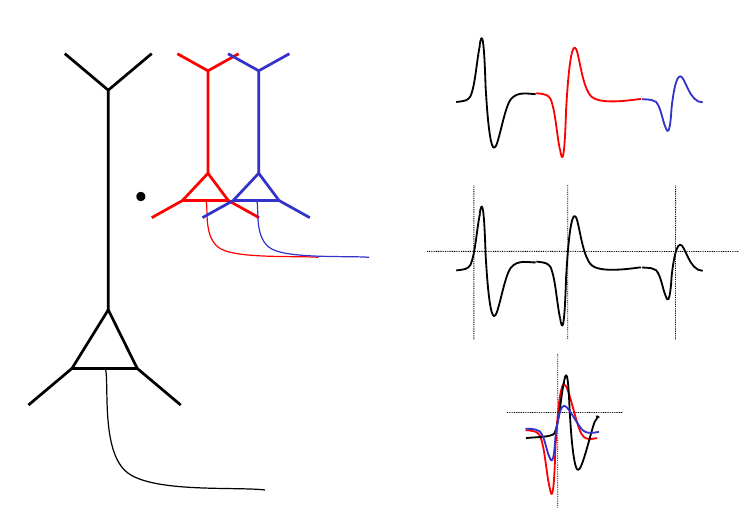
\includegraphics[keepaspectratio, width=\linewidth]{img/2_lfp_mur.png}
         \caption{When the meassuring electrode is placed not very close to one neuron but to multiple neurons, the recorded signal contains contributions from many neurons with their magnitude depending on the distance from the electrode and on the frequency (see below).}\label{mur}
        \end{subfigure}
         \begin{subfigure}{0.45\textwidth}
          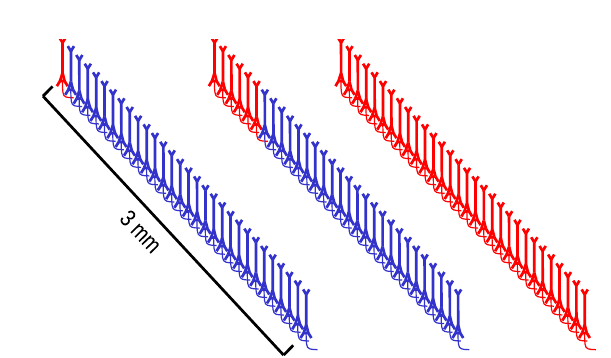
\includegraphics[keepaspectratio, width=\linewidth]{img/2_lfp_origins.png}
          \caption{Depending on the distance of the neuron, different frequency components of the neurons contribute: When the neuron is close, also high frequency components are contributing, while whith increasing distance only lower components do. This is due to the size of the generating source: The field generated by single APs is rather small, while synchronous firing of a population causes the electrical field to extend further.}\label{origins}
         \end{subfigure}
        \end{figure}

        The size of the population that is recorded depends on the recording setup, e.g. the distance between two electrodes, the electrode position and the size of the electrode itself. The broadest scale signals like electroencephalographies (EEGs) only allow the analysis of large groups of populations. To summarize: With decreasing spatial resolution, the aggregation of the currents emitted by the neurons increases, i.e. the signal is more ambiguous to interpret in terms of the sources~\autocite{einevoll2013modelling, herreras2016local}. This yields information on a more global scale or that is more network-oriented. \\
        On the other hand with an increase in spatial resolution, the neccessary temporal resolution or the frequency at which the signal has to be sampled to caputre the information has to increase to capture all phenomena. \\
        Thus for single unit recordings it makes sense to detect action potentials by using an absolute threshold, while for multi-unit recordings, a threshold can be used to detect peaks in the signals but they correspond by no means to action potentials but rather to a high synchronity in the recorded neural population~\autocite{herreras2016local}.
        \begin{figure}
         \begin{center}
            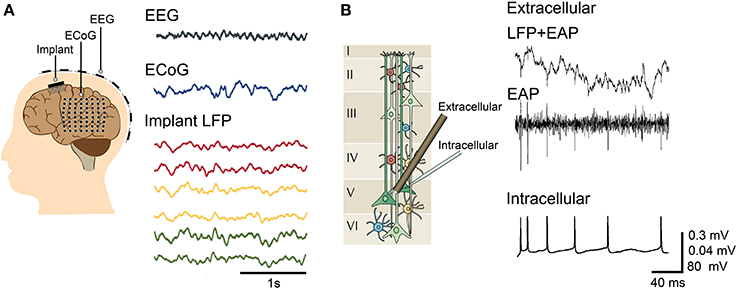
\includegraphics[keepaspectratio, width=0.45\textwidth]{img/2_lfp_scales.jpg}
         \end{center}
         \caption{\textbf{A:} Different LFP recording methods that operate on a broader spatial scale. \textbf{B:} Extra- vs. intracellular recordings.  ~\autocite{10.3389/fnins.2014.00423}}
        \end{figure}

        Bursting activity can be detected for single-unit recordings by different methods ranging from using fixed threshold parameters based on burst duration, min. number of spikes per burst, maximal inter-spike interval (ISI) within a burst, and the like, over methods using the logarithmic inter-spike interval histogram to derive a threshold or the cummulative moving average of the ISI to methods using statistical models, e.g. the posisson model~\autocite{cotterill2019burst}. \\
        For MURs this does not make a lot of sense. LFPs contain waveforms with large amplitude and a large duration, which invalidates approaches using spike-intervals. Detecting the bursts of a population by a fixed theshold is suboptimal too, as the signals of the population can cancel out when firing asynchronously and the amplitude of a waveform differs significantly depending on the placement of the electrode(s). Finally statistical methods often make assumptions which are not neccessarily true. For example the Poisson Surprise method assumes that spike-trains are Poisson distributed~\autocite{cotterill2019burst}.

        For MURs we need other means of analysis which are laied out in the next section.

    \subsection{Multi-Electrode Arrays}
        The data that is supposed to be analyzed was recorded using multi-electrode arrays.
        A micro-electrode array consists of many small open-gated field-effect transistors or oxide-semiconductors assembled into an array to record local field potentials extracellulary.~\autocite{10.3389/fnins.2014.00423}.
        Along with the electrodes itself and a chip holding and wiring them together, MEA systems include analog signal processing subunits to allow for controlling the sampling rate and stimulation parameters.
        A picture of such a MEA system is shown in figure \ref{mea}.
        \begin{figure}
         \begin{center}
          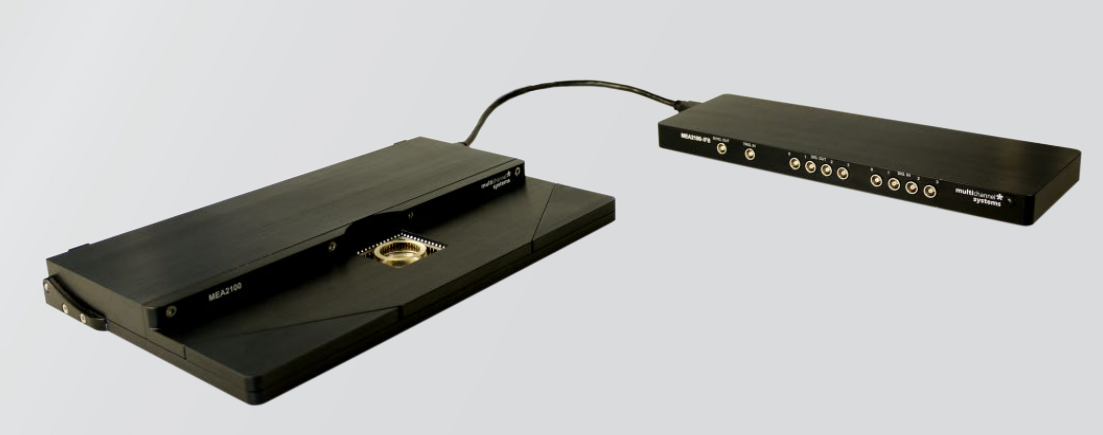
\includegraphics[keepaspectratio, width=0.45\textwidth]{img/1_setup_mea.png}
         \end{center}
         \caption{A multi electrode array head stage (right) and interface board (left). Model: MEA2100-System by Multi Channel System (MCS) GmbH.}\label{mea}
        \end{figure}

        In general this allows for the recording of both LFPs and extracellularly recorded APs (EAP).
        Depending on the electrode distance, the EAPs contribute a smaller or larger share to the signal and ultimatively control the resolution of the MEA.
        Those with an electrode distance of the size of less than a soma can be used for EAP recordings while MEAs with larger distances rather record LFPs with only smaller contributions from EAPs.
        A new class, the so called HD-MEAS are complementary metal-oxide-semiconductor-based (CMOS-based).
        These are even able to record with sub-cellular resolution.

        Both in-vivo and in-vitro setups can be realized with these devices --- here we focus on in-vitro set-ups.
        One possibility is to meassure cultured cells, either by cultivating them on the chip directly or by plating previously cultered cells to the chip.
        The former preserves the connections within the cultered network, while the latter destroys inter-cellular connections, causing the neurons to spontaneously form networks~\autocite{POTTER200117, gross2006emerging, POTTER200149}.
        As the amount of cells and cell types is smaller and the structure of the cells is poorer compared to slices, the data is more homogeneous. \\
        Another possibility is to plate a brain slice.
        Here the connectivity in the network is preserved in 2D and depending on the thickness of the slice in small amounts also in three dimensions. This is of course only to a certain degree as the slicing process itself is degrading the connectivity.
        Thus data recorded using slices is more heterogeneous and corresponds better to the in-vivo case~\autocite{soussou2006mapping, gross2006emerging}.
        A picture of such a brain slice plated on a MEA is shown in figure \ref{setup}.
        \begin{figure}
         \begin{center}
          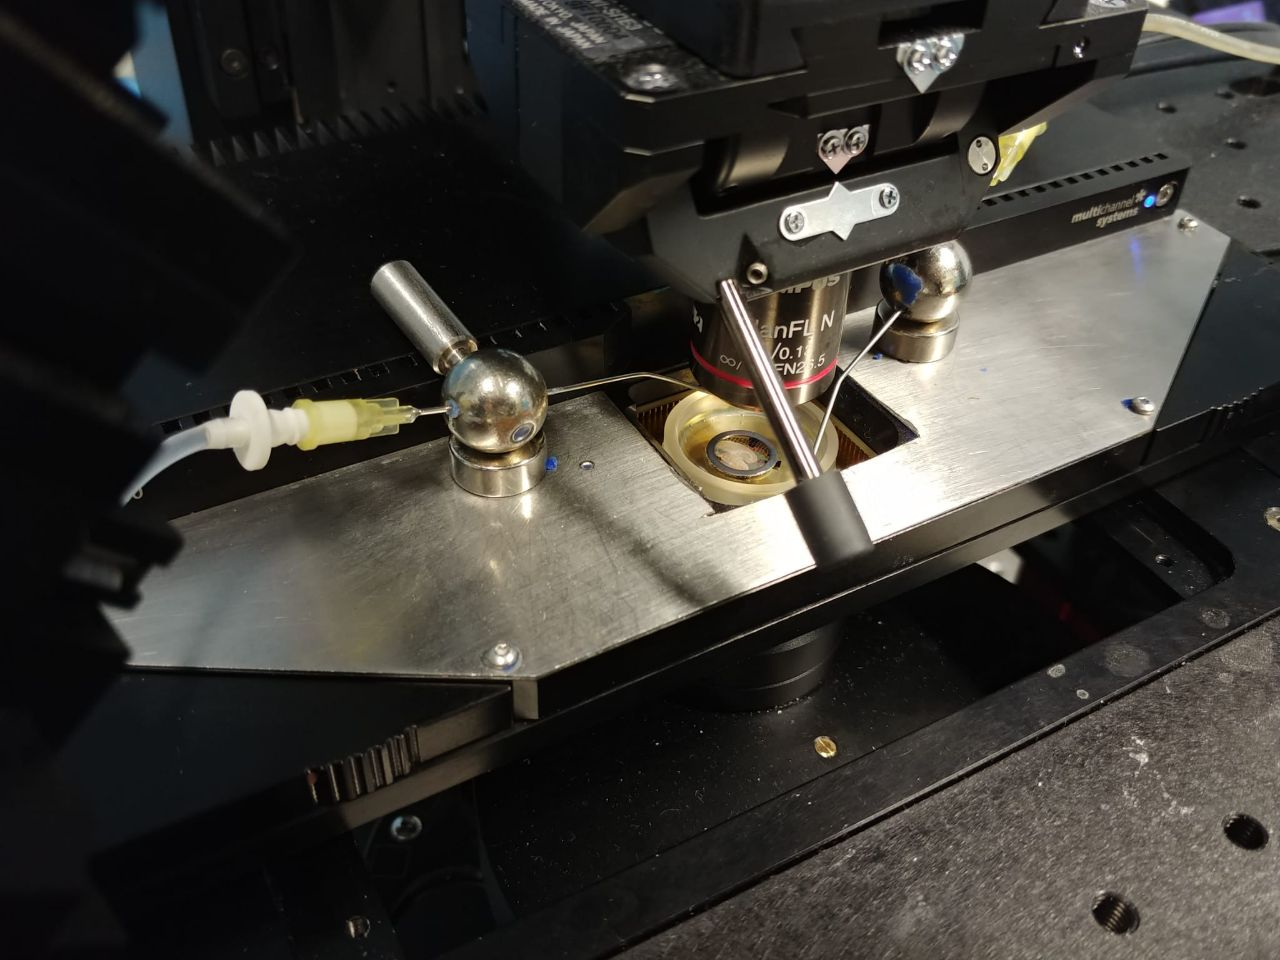
\includegraphics[keepaspectratio, width = 0.45\textwidth]{img/1_setup_close.jpg}
         \end{center}
        \caption{Setup to record LFPs from a mouse brain slice using a MEA.}\label{setup}
        \end{figure}

        The figure \ref{slice} shows a light microscopy image of the brain slice on the MEA.
        Notice the black dots, which are the electrodes.
        \begin{figure}
         \begin{center}
          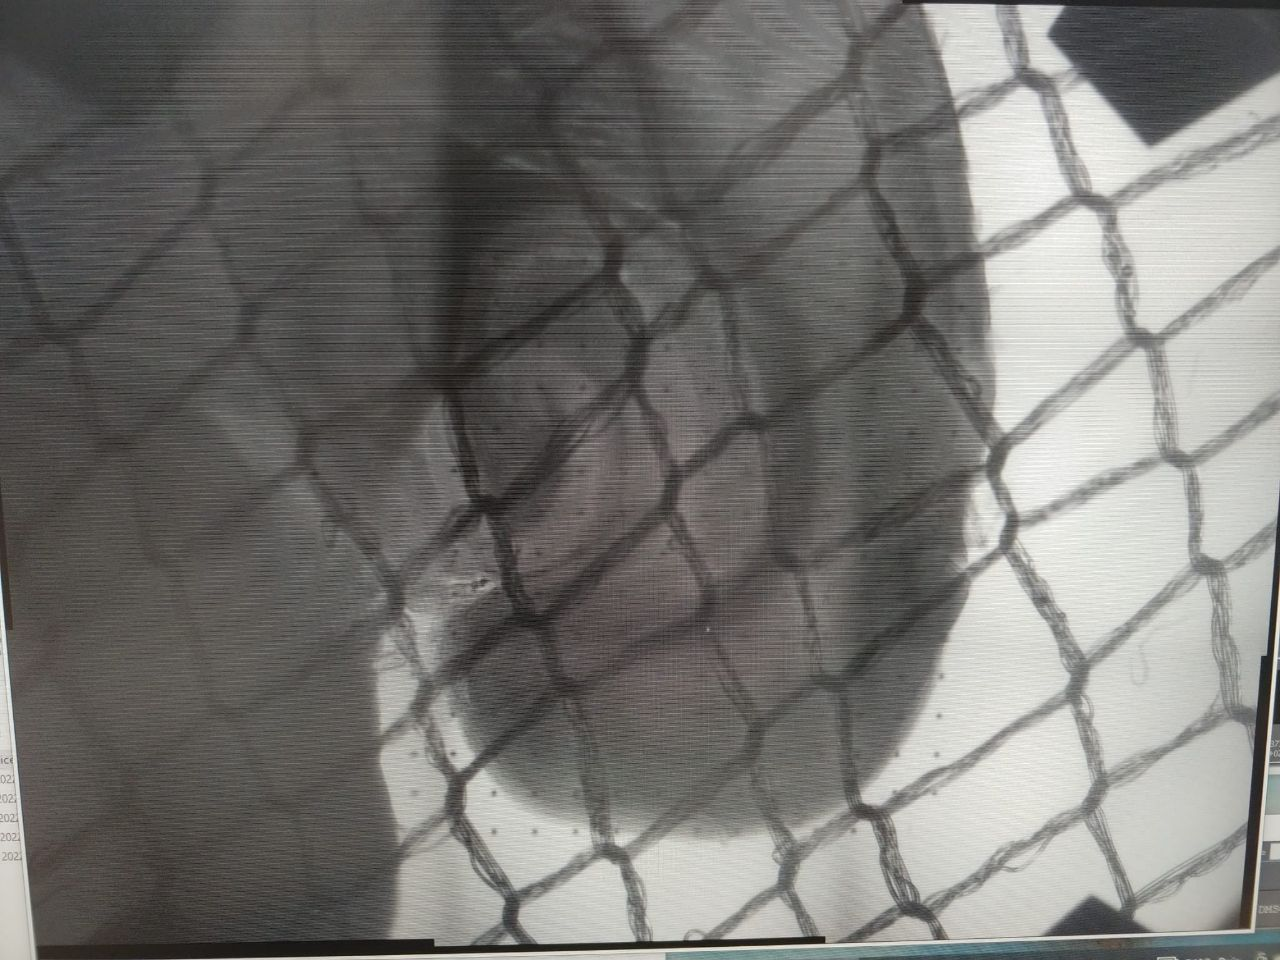
\includegraphics[keepaspectratio, width = 0.45\textwidth]{img/1_setup_slice_.jpg} \\
         \end{center}
        \caption{Light microscopy image of the mouse brain slice taken in the setup above.}\label{slice}
        \end{figure}

    \subsection{Existing Analysis Software}
        There are multiple frameworks for analyzing local field potentials~\autocite{unakafova2019comparing}.
        Most prominently there are the FieldTrip toolbox for Matlab and the MNE toolbox for Python, which both focus on LFPs recorded with EEG, MEG, ECOG and the like\autocite{gramfort2014mne, oostenveld2011fieldtrip}.
        Their spatial resolution is orders of magintude lower compared to MEAs, thus many methods provided by these and similar packages are unsuitable. \\
        Other toolboxes rely on spike sorting only, i.e. do not take the temporal structure of the signal before and after a waveform into account (e.g. Brainstorm~\autocite{tadel2011brainstorm}).
        Toolboxes which only focus on (binary) spike trains fail to capture the magnitude of certain patterns, like waveforms.
        These have often a large amplitude and are rather slow compared to e.g. an AP.
        They appear often at the end of an an epileptoform seizure, and with a focus on binary spikes this information is ignored. \\

        The Python package Elephant provides a set of useful functions, like current source density analysis and the computation of Granger causality. It also provides means to analyze the features of a waveform.
        So far elephant does not provide a graphic user interface (GUI).

        A comprehensive review of many toolboxes is laied out in ~\autocite{unakafova2019comparing}. \\

        The toolbox provided by Multi Channel System uses a single threshold across all electrodes which does not suffice to caputre the heterogeneity across different electrodes or groups of electrodes.
        Also it does not provide means to analyze seizure-like behavior.

        There are very few pieces of software which specifically focus on the analysis LFPs during seizures.
        One which does is the Xenon LFP Analysis Platform which provides a GUI, analysis and visualization tools.
        However the focus is set on HD-MEAS, thus focusses on APs and only support their own data format.
        For example Xenon uses a single user-defined threshold to detect peaks in the signal.
        In lower resolution MEAs when recording from a slice, the magnitude of spikes varies across electrodes.
        The seizure detection method relies on spikes and the spectrogram with a spectral power threshold and a user-defined duration minimum which defaults to 10s.

\section{Methods}
\subsection{Task Definition}
	The task is to analyze data recorded with the Multicannel systems MEA2100-HS256 headstage and the Multichannel systems 256MEA200/30iR-ITO chip of a wild type and a SCN1A mutant A1783V.
	The software system should incorporate methods that assist in the inspection and quantification of differences in neural activity between A1783V mutants and wild type mice during baseline and seizure/seizure-like conditions.
	Concretely it shall assist in answering the questions how far, how fast, with what magnitude and with which subcomponents a seizure-like firing activity spreads upon the presentation of a stimulus with NMDA, 4AP and Mg deprived solution.

	The system shall enable the visual exploration of data, the selection of channels and the time window of interest, provide plots of well-established transformations like the Fourier transform or a spectrogram, the detection of peaks and bursts in the signal, the computation of functional connectivity between specified electrodes with measures like transfer-entropy or Granger causality, the visualization of raw data, computed transforms and quantities and the spreading behavior of seizure-like events.

	\subsection{Constraints}
		\begin{itemize}
			\item The electrodes of this MEA systems are $200\mu$m appart, such that it is at least extremely difficult and ambiguous to identify single spikes.
			Thus all methods that rely on spike-based meassures shall be avoided in the first place.
			At a later stage however this feature may be added to support the analysis of data generated by CMOS-based MEAs.
			\item The computational and temporal capactiy for this project is limited, that is the system shall be able to execute a full data analysis pipeline in less than 24 hours on the whole dataset.
            \item a MEA has many electrodes, here 252. Data is sampled at sampling rates as high as 25 kHz and the signals are heterogeneous when comparing different electrodes. This means that each data set is very large. A 2 minute recording with sampling rate 25 kHz has a compressed size of $~1$ GiB and an uncrompressed size of $~3GiB$.
            Further, as we use brain slices as probes, the data is very heterogeneous which prohibtis a reduction in dimensionality by means of modelling multiple similar enough electrode by a common variable.
            \item 	In our setting, data has been recorded from a MEA with 200 $\mu$m electrode spacing which does not allow for the detection of action potentials.
			Thus non-spikes based analysis meassures shall be used.
			Also the threshold parameter varies per electrode, such that peaks should be detected independent of constant thersholds. \\
		\end{itemize}

		Existing software solutions are either proprietary, vendor specific, scale specific or not flexible enough for our purpose. Thus to fullfill the task, a new piece of software shall be implemented, which provides similar functions as both the proprietary toolbox by Multi Channel System and the Xenon LFP analysis platform together.

	\subsection{Proposed Software Design}
		All of the subsequent steps are implemented using the Dash framework like in Xenon's platform, with the addition of Bootstrap extensions provided free and open source by Faculty AI.
		This enables that each step is carried out in a separate subpage.
		As many functions as possible shall be implemented as wrappers of other libraries like SciPy~\autocite{2020SciPy-NMeth} with GUI integration.
		Further as Dash serializes all plotted data into a Json object which can get very large for large amounts of data, this imposes a high memory load on the hardware system.
		Thus Matplotlib~\autocite{Hunter:2007} is used to render all plots which do not require interaction. \\

		These conditions suggest the usage of the model-view-controller paradigm, where the model contains data and metadata, while the controller provides means to manipulate data/the model and the view provides a visualization of the model/manipulated data.
		This is empoyed with a pipeline: First the data is imported, then the desired channels and time window are selected, next the signal is filtered and downsampled (to speed up computaitons).
		Finally transformations and analysis methods are applied and their result is visualized.

		\textbf{Loading \& Focussing}
            The format that the MEA system by Multi Channel System uses is based on the Hierarchical Data Format 5 and a library to work with it, called McsPyDataTools, is provided by the vendor.
			Like in Xenon's platfrom, electrodes are selectable dynamically and the current selection is visualized interactively thanks to Dash. Also, the time region of interest can be specified and the selected data can be visualized via Matplotlib on request.
			\begin{figure}
			 \begin{center}
			  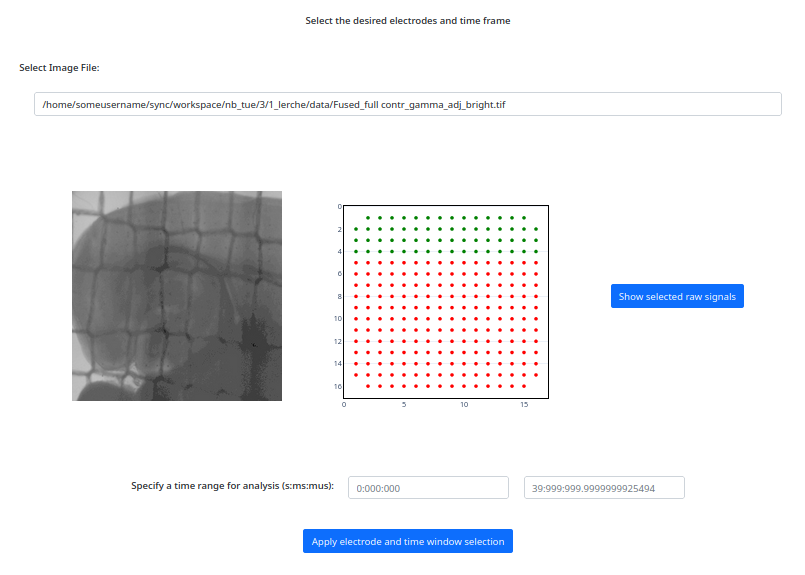
\includegraphics[keepaspectratio, width=\linewidth]{img/4_select.png}
			 \end{center}
				\caption{A screenshot of the selection screen. On the very left, an image of the recorded slice can be uploaded for the used to estimate which electrode corresponds to which region in the slice. Next to it, the electrode grid with selected electrodes is rendered. On the very right, there is a button that triggers the plotting of the selected signals. Finally on the bottom, we can see the input fields for the time window to be set.}
			\end{figure}

		\textbf{Preprocessing}
            The signals can be filtered using a band-pass filter designed with either the method of Butterworth or Chebyshev~\autocite{williams2006electronic}.
            Additionally, the data can be downsamplable to a user defined sampling rate.
            For that the SciPy function decimate is used which first applies an anti-aliasing filter/low-pass (order 8 Chebyshev type I) and then downsamples the signal.
            Further, electric humming with a frequency of 50 Hz (EU) can be removed.
            All filter functions use the implementation by SciPy via cascaded second-order sections~\autocite{2020SciPy-NMeth}.

			\begin{figure}
			\begin{subfigure}{0.45\textwidth}
			\begin{center}
			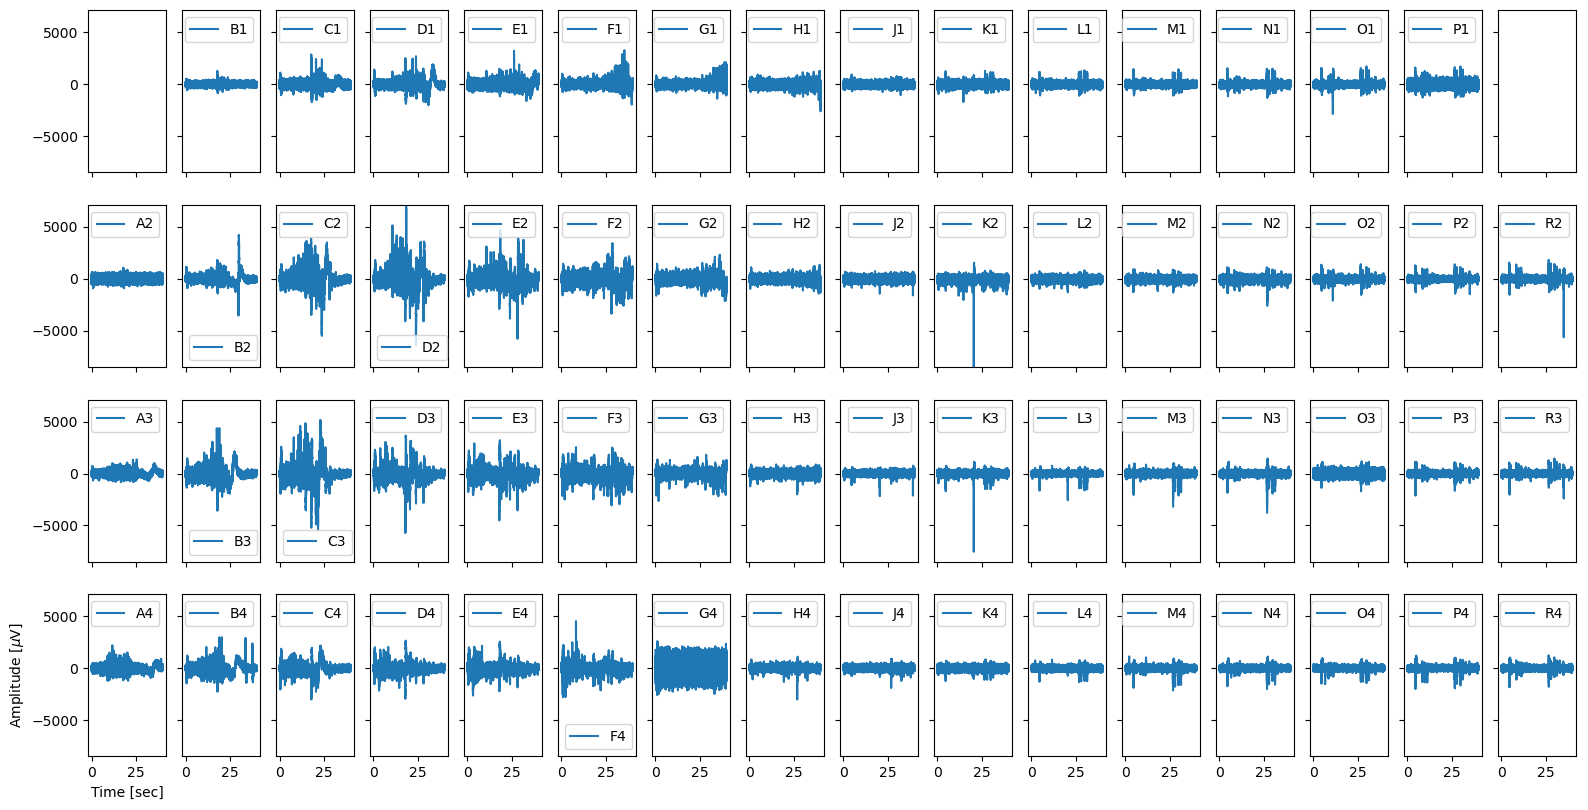
\includegraphics[keepaspectratio, width=\linewidth]{img/4_raw.png}
			\end{center}
			\caption{The raw signals can be plotted and are arranged in the plot like the electrodes on the grid.}
			\end{subfigure}

			\begin{subfigure}{0.45\textwidth}
			\begin{center}
			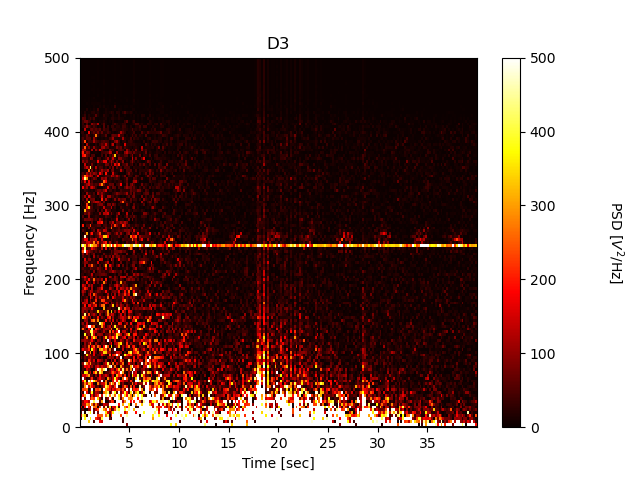
\includegraphics[keepaspectratio, width=\linewidth]{img/4_spectrogram.png}
			\end{center}
			\caption{A spectrogram of one electrode signal.}
			\end{subfigure}

			\begin{subfigure}{0.45\textwidth}
			\begin{center}
			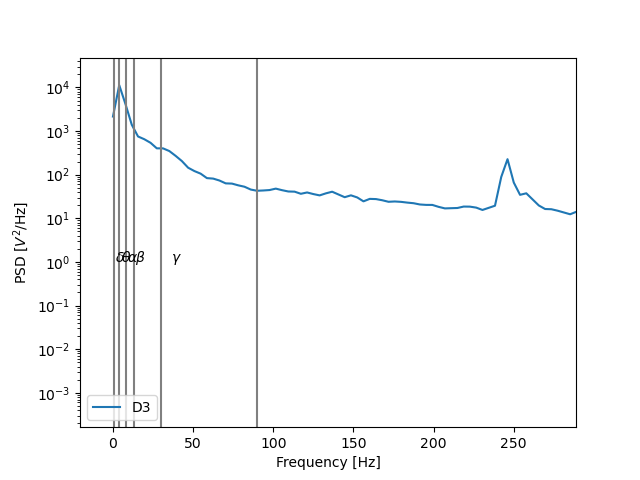
\includegraphics[keepaspectratio, width=\linewidth]{img/4_psd.png}
			\end{center}
			\caption{The power spectral density of the same signal.}
			\end{subfigure}
			\end{figure}

		\textbf{Transformations \& Analysis}
            The libraries Numpy~\autocite{harris2020array}, Scipy~\autocite{2020SciPy-NMeth}, PyIF~\autocite{0f6676b4112b417ba70c97456553d691} and FOOOF~\autocite{donoghue2020parameterizing} are used to implement the various signal processing and statistics procedures.
            Power spectral densities using Welch's method~\autocite{1161901}, the root mean square~\autocite{oppenheim1999discrete}, the moving average, the envelope using the Hilbert transform~\autocite{king2009hilbert}, spectrograms using short time fourier transform~\autocite{oppenheim1999discrete}, the decomposition of the signal into periodic and aperiodic components using FOOOF, transfer entropy using PyIF, and algorithms to detect peaks and bursts with the before mentioned contraints are implemented. The algorithms will be described in the next subsection. Additionally statistics to quantify a burst can be calculated and summarized for the longest brust across different electrodes.

		\textbf{Visualization}
            The before mentioned transforms and quantities are visualized using Matplotlib.
            Additionally, the presented piece of software is able to visualize electrodes over time.
            For that the signal can be both binned (such that there are less frames) and slowed in order to capture the changes in signal distribution across electrodes.
            Finally a raster plots with color-coded amplitude and a PSTH can be generated, too.
			\begin{figure}

			\begin{center}
			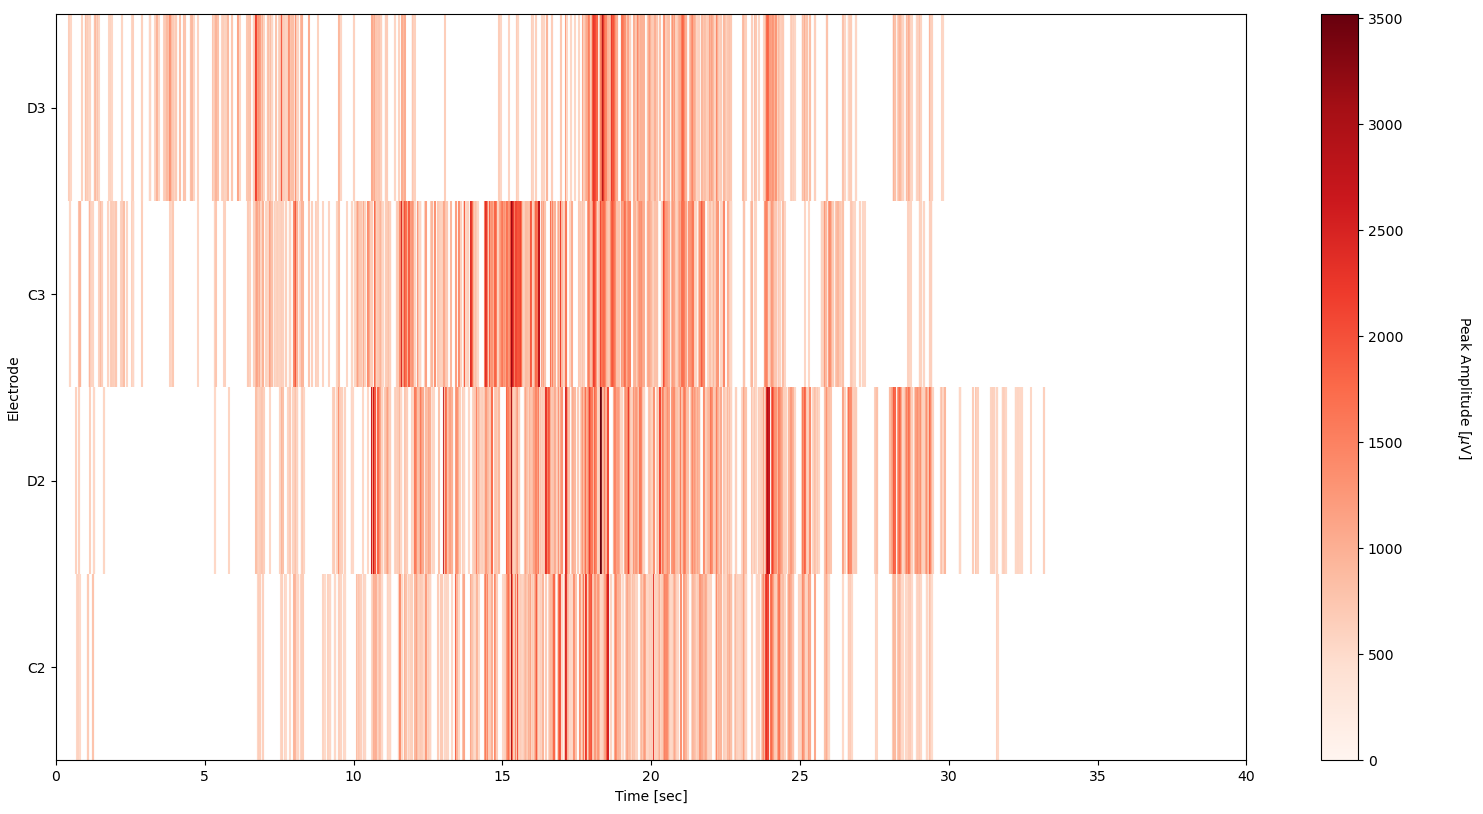
\includegraphics[keepaspectratio, width=\linewidth]{img/4_raster_avg.png}
			\end{center}
				\caption{A rester plot of the detected peaks. The color encodes the amplitude of them.}
			\end{figure}



\subsection{Algorithms}
    \textbf{Peak Detection by Amplitude} is the default methods to detect peaks. SciPy provides a function called \texttt{find\_peaks} which detects points in the signal that are above a threshold. As already mentioned setting one global threshold for all electrodes will yield a low quality result, where peaks of electrodes with a weaker signal are in general not detected (as below the threshold). To mitigate this, we use a baseline file to extract the standard deviation per electrode and globally. We then use a weighted sum of the global and the electrode-local standard deviation.
    \begin{figure}
     \begin{center}
      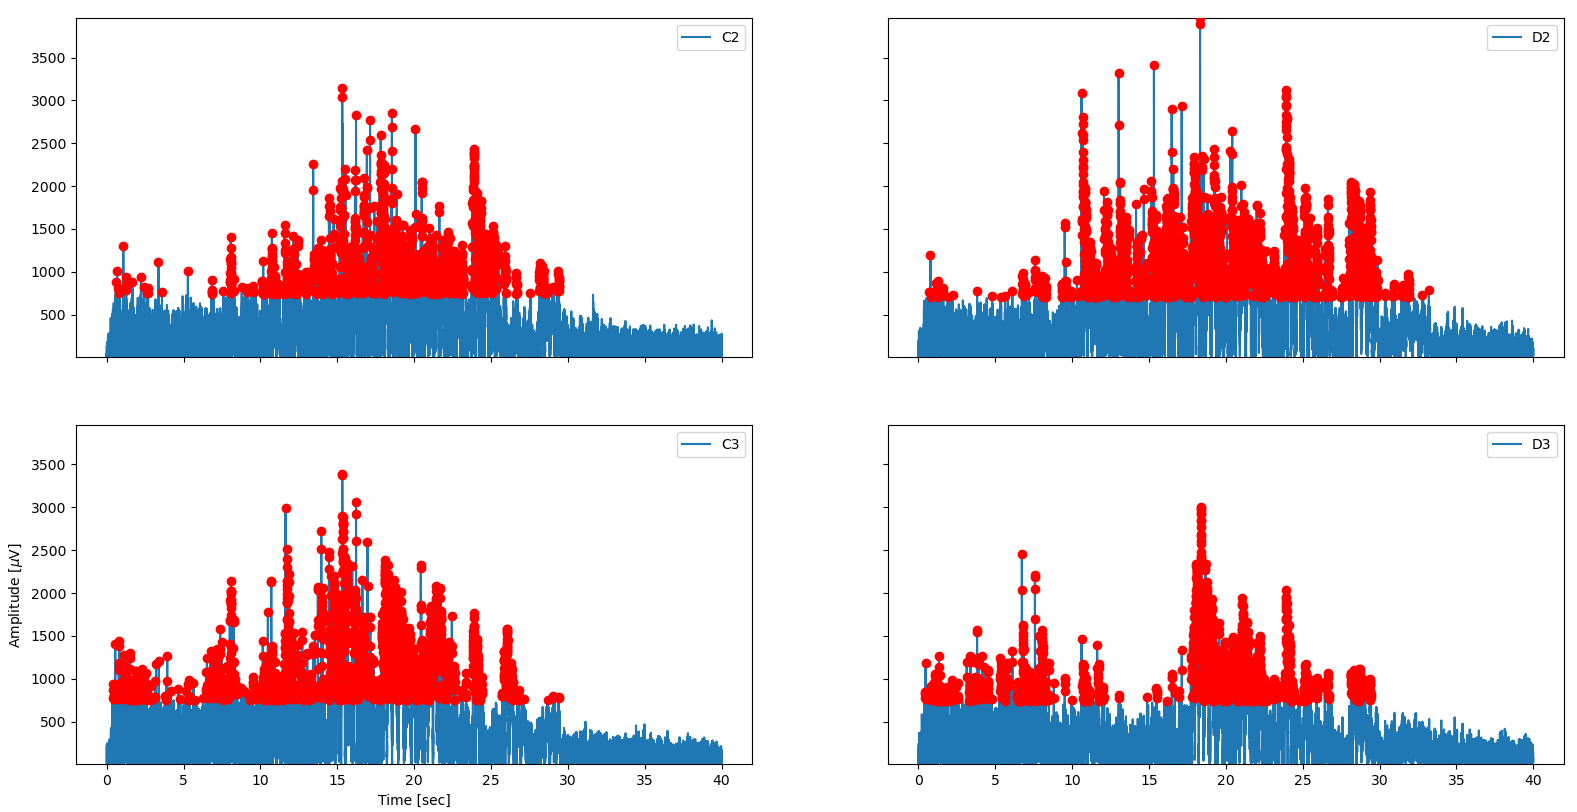
\includegraphics[keepaspectratio, width=\linewidth]{img/4_peaks_amplitude.png}
     \end{center}
		\caption{Peaks detected by the threshold method. Every single peak is detected reliably.}
    \end{figure}

    \textbf{Peak Detection by Moving Average} of the absolute signal can be used to avoid relying on the amplitude of the signal at one specific point in time but rather over time windows. For that we compute the moving average of the signal with a small window size (e.g. $0.1\%$ of the signal). Then we compute the moving average of the basline signal and compute the standard deviation both per electrode and globally. \texttt{find\_peaks} is then again used with a weighted sum of the local and the global standard deviation of the moving average as a threshold. This method detects peaks that happen in a short amount of time best, while not detecting a short single peak without an increase in previous or following activtiy, thus excluding isolated spontaneous activity.
	\begin{figure}
     \begin{center}
      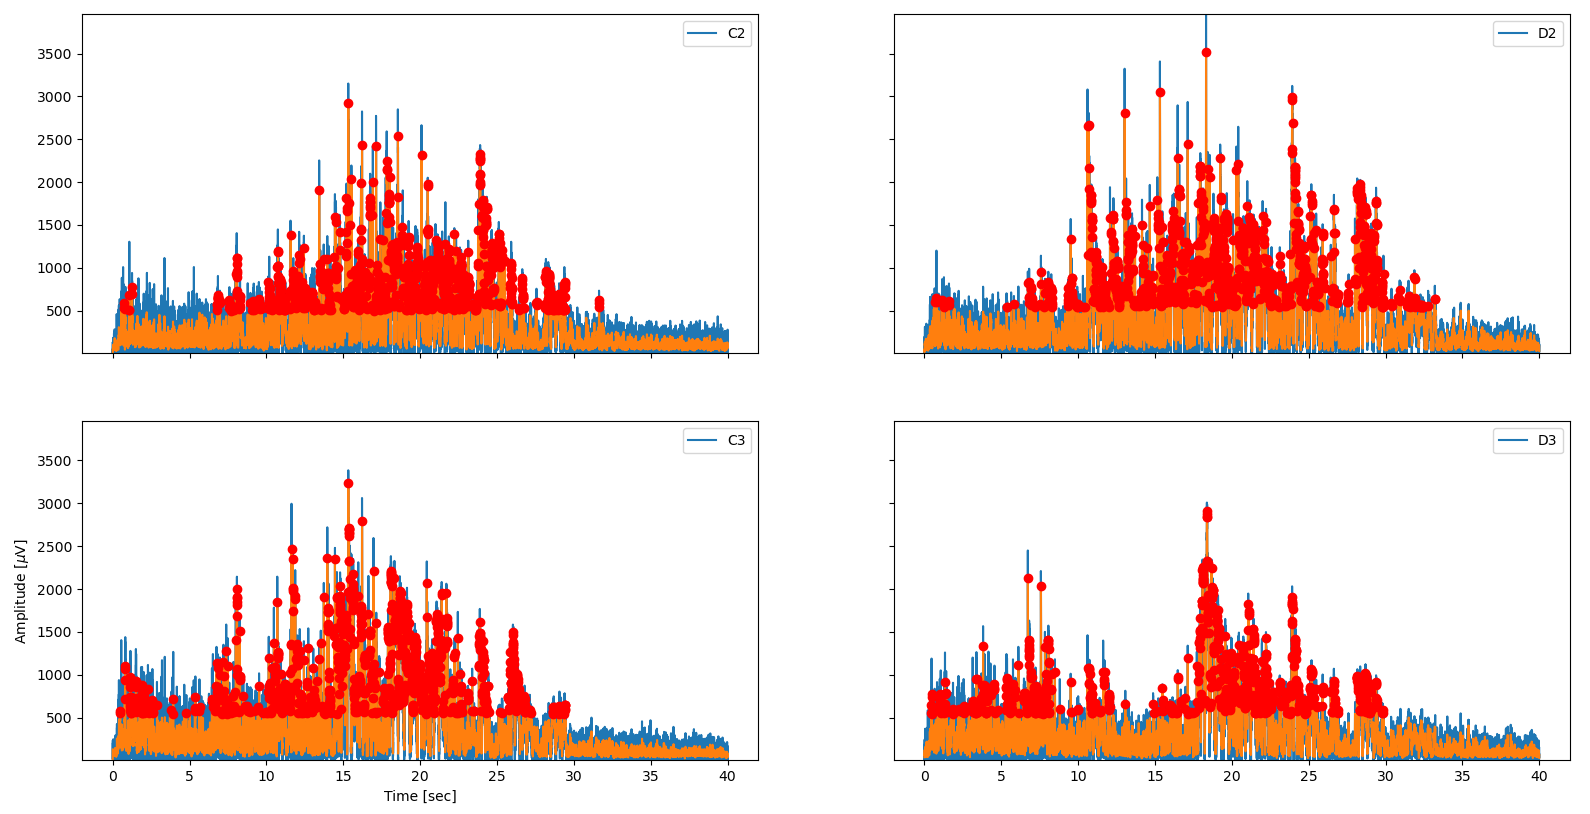
\includegraphics[keepaspectratio, width=\linewidth]{img/4_peaks_avg.png}
     \end{center}
		\caption{Peaks detected by the moving average method. Peaks with little activity in the vincity are not detected.}
    \end{figure}

    \textbf{Burst Detection by Moving Average} works similar to the approach before: calculate the moving average of the absolute signal and a baseline --- this time with a window size as large as e.g. $5\%$. Then find the points where the signal crosses the threshold both rising and falling and mark the points in between as burst. For the detection of seizure-like events, only the longest burst is selected.
    The idea behind this is that taking a larger window will result in the detection of parts of the signal where there is a lot of activity in the vincity, such that only highly oscillating regions are detected.
	\begin{figure}
     \begin{center}
      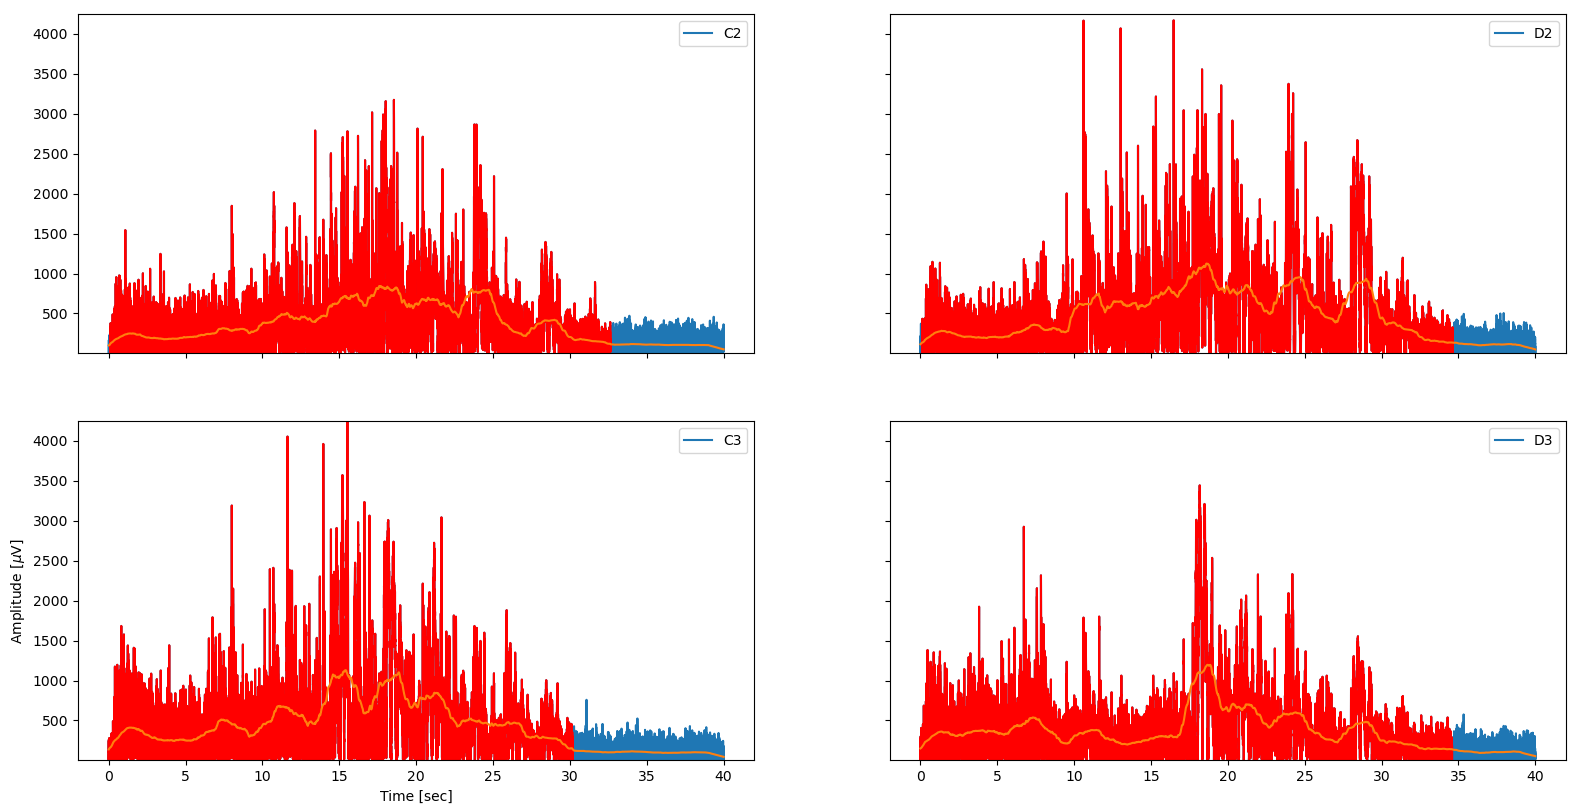
\includegraphics[keepaspectratio, width=\linewidth]{img/4_bursts_avg.png}
     \end{center}
		\caption{Epileptoform bursts detected by the moving average method. }
    \end{figure}


    \textbf{Burst Detection by Moving Standard Deviation} uses the insight that with bursting activity, the standard deviation increases for that region of the signal, while if there is no bursting activity it decreases or stays low.
    The computation for this ``moving standard deviation'' is computed as follows per electrode:
    First the mean of the signal is calculated, then it is subtracted from each data point in the signal, and this difference is squared.
    \[ s^2_{ij} = {x_{ij} - \overline{x_i}}^2 \]
    The moving average of this quantity is then computed and the root of the result is taken.
    \[ s_{ij} = \sqrt{\text{moving average}(s^2_{ij})} \]
    This quantity does not correspond to the moving standard deviation as defined in the literature.
    Again the weighted sum of the standard deviation of the baseline locally and globally is used as threshold along with \texttt{find\_peaks} on the computed quantity and only the longest peak is extracted for the detection of seizure-like events.
    	\begin{figure}
     \begin{center}
      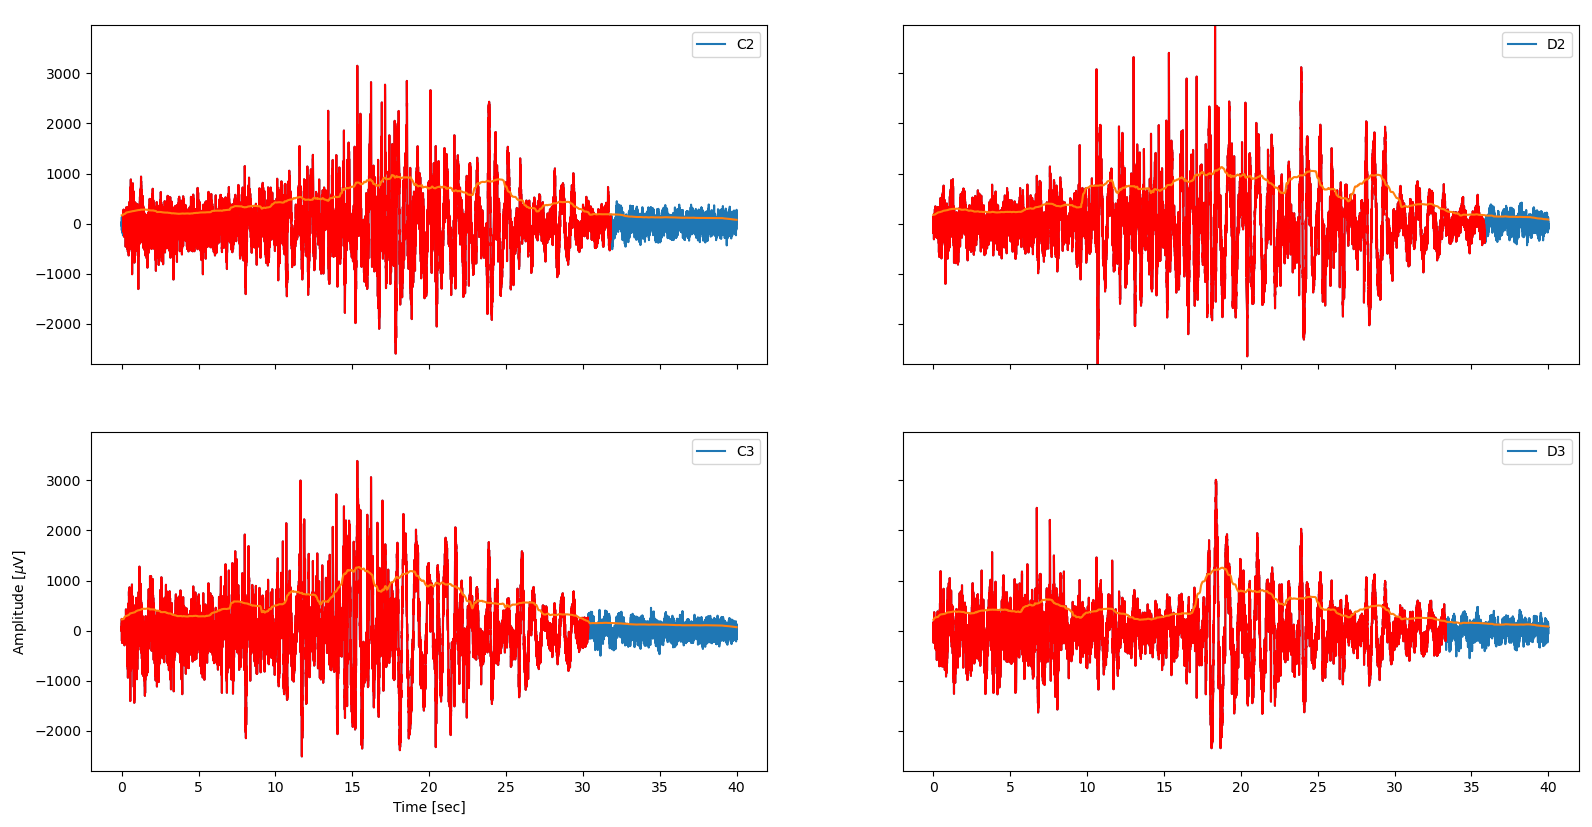
\includegraphics[keepaspectratio, width=\linewidth]{img/4_bursts_std.png}
     \end{center}
		\caption{Epileptoform bursts detected by the moving standard deviation method.}
    \end{figure}

\section{Discussion}
As time was critical for the project, the software is limited in multiple ways:
\begin{itemize}
 \item So far there is no possibility to assess multiple groups in one run of the pipeline but the whole pipeline needs to be executed once per group.
 \item Transfer Entropy is a meassure that intuitively should specify how good one signal is predictable by another signal.
 For it's computation the user needs to define an embedding which corresponds to the amount of previous data of the signal to predict the other one.
 The larger the value, the slower the computation.
 As we have $3M$ data points for a non-downsampled signal of 120s in length, at least a couple of dozend points should be considered.
 This however leads to runtimes of multiple hours to days depending on how large this embedding value is set. \\
 An alternative approach would be to use current source density estimation in a spatio-temporal frame, i.e. locate sources and sinks across different frames in time and across different electrodes in space~\autocite{nicholson1975theory}.
 \item Many of the operations carried out are parallelizable which is currently not implemented.
 \item So far only the 256 electrode MEA is supported. Other systems like HD-MEAs for slices or CMOS MEAS for cell cultures are to be supported as of now, as well as other kinds of systems like deep brain stimulation electrodes or single microelectrodes.
 \item Some parameters are not yet configurable on the GUI.
\end{itemize}
In order to asses the correspondence of in-vitro recorded data with the in-vivo dynamics, a correlation analysis between the MEA recordings and e.g. in-vivo recordings via a tetrode seems to be promising.
Further the alignment and/or fusion of the MEA data with 2-Photon CA$^{2+}$ will yield a richer, multi-modal data set.



\section{Conclusion}
The analysis of MEA recorded LFPs poses unique challenges that haven't been addressed in in a unified piece of software, that is accessible to a broader audience. Many current solutions do not provide a GUI, are proprietary and bound to certain vendor formats, qualitatively insufficient or do not address the right spatial scale. \\
To resolve this for the specified setting a toolbox has been implemented which heavily draws from functions implemented in popular or specialized libraries, hooked into a GUI and the output is visualized.
Two different approaches were implemented to detect peaks.
Different algorithms have been used to circumvent the usage of binary events for burst detection and to reliably account for peaks of all durations in the burst. Statistics that characterize the epileptoform burst and quantify the spread of the seizure-like event. \\
Current source density analysis provides a mathematical framework to refine the quantification of the spreading event both in magnitude and speed.
Other sources of data can be merged into one large mutli-modal data set that allows to add further insights into the network activity during a seizure and dimensions to the data analysis.

\hspace{0pt}\vfill
\section*{Acknowledgements}
\vfill\hspace{0pt}
I'd like to thank Nikolas Layer, Dr. Thomas Wuttke and Dr. Ulrike Hedrich-Klimosch for the time and effort they spend to supervise, to teach and to help me. 
\newpage

\printbibliography
\end{document}
